	
\subsection{Current state of own research and professional competences for the project}
% 1000 words

\begin{figure}[h]
	\centering
	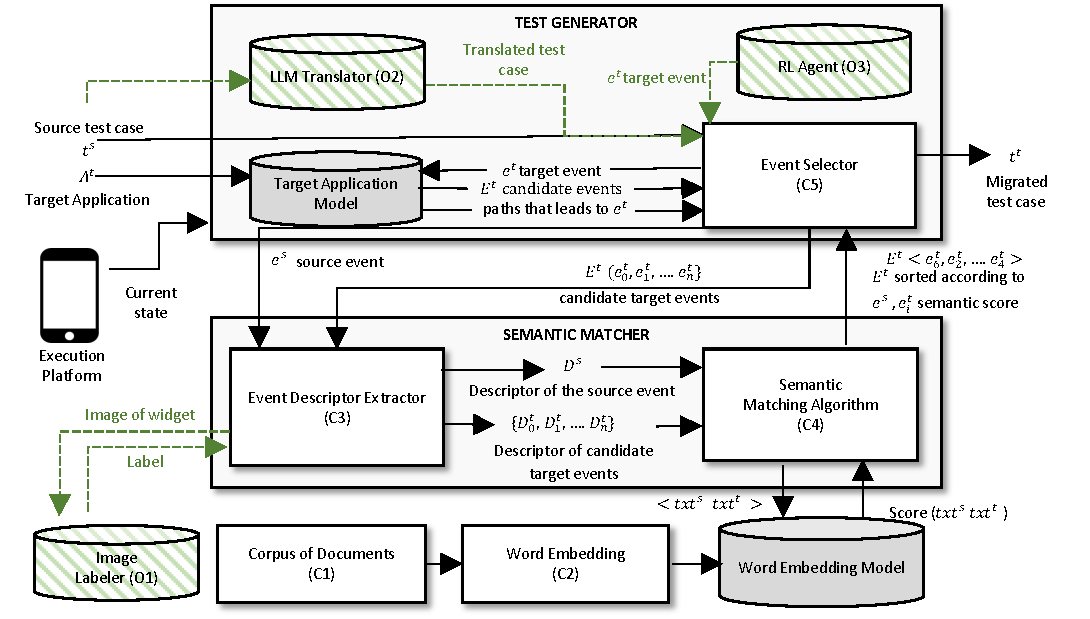
\includegraphics[width=\textwidth]{images/architecture.pdf}
	\caption{\testreuse architecture and project objectives}
	\label{fig:architecture}
\end{figure}

%Test Reuse architecture
We started our study of \testreuse  by full replication of experiments of state-of-the-art  \testreuse approaches, and careful inspection of their source code that is publicly available. 
We considered \craftdroid~\cite{lin:craftdroid:ASE:2019}, \atm~\cite{behrang:apptestmigrator:ASE:2019}, and \adaptdroid~\cite{Mariani:Adaptdroid:AST:2021} in our study.
After reviewing state-of-the-art approaches, we proposed a general \architecture that encompasses common components of \testreuse approaches and their interaction. 
Figure~\ref{fig:architecture} shows our proposed architecture.
Components C1, C2, C3, C4, C5 are the components that already exist in the current approaches and O1, O2, O3 (in hashed green) are realization this proposal objectives. 

% Test Ruse work flow
\bigskip
\testreuse approaches include two coarse grain parts \generator and \matcher.
\generator receives a source test case  and a target application, then it iterates over events available in source test case. 
For each event in the source test case \generator considers a set of candidate events from the target application and queries \matcher.
\matcher sort the target candidates based on their semantic similarity to the source test case.
\generator selects from sorted candidates and executes the event to transport the current GUI state to another state. 
After, iterating over all the source test cases each selected events in the target application comprise the migrated test case.

\bigskip
In more detail, the \testreuse work flow starts with receiving the target application $A^t$.
The \generator statically analysis the application and creates a \tam and updates the model as it progress in migrating the source test case $t^s$.
The \selector (C5) incrementally migrates the $t^s$ to generate a test case $t^t$ for $A^t$.
To do so, the \selector iterates over source events in the $t^s$ and for each source event $e^s$ select an event in the target application that is semantically matched with the source event.
\selector retrieves a set of target candidate event $E^t$ from current state of the \tam. 
If the \selector selects an events from the \tam, that means it should take few stepping events to reach an state where the selected event is available. 
\selector queries the \tam to find a path to the event of in a state other than the current one. 
\selector queries the \matcher to  sort the $E^t$, then it selects an event from the . 

\bigskip
The \matcher receives the set of target  candidate events $E^t$ and the source event $e^s$ and \ede (C3) extracts textual descriptors $D$ of the events. 
\sma receives both descriptors of the source event $D^s$ and target candidates $\{D_0^t, \dots D_n^t\}$ and queries the \wem to score textual attributes available in the descriptors. 
Finally, \sme aggregates the scores of attributes and sort the target events $E^t$ based on their similarity to the  source event $e^s$.
\wem is built once for all from training a \we techniques (C2) on a given \corpus (C2). 
\we techniques create models that encodes words and sentences to vectors that represent semantic distance of them in the \corpus.


\bigskip
Components of \testreuse can be implemented in different ways.
We call concrete implementation of each component an instance of the component.
Each combination of instances for the semantic matching components (C1-C4) yield a unique configuration of matching that we call \smconfig
Basically, each configuration answers semantic queried differently --  a query is a source event  and a set of target candidates in which the source event should be matched with the target candidate. 


\bigskip
We understood that Semantic Matching is an important part of \testreuse and to carefully study its limitation and possible ways for improvement we first studied semantic matching in isolation from \testreuse~\cite{mariani:SemFinder:ISSTA:2021}.  
We consider instances that we identified in the state-of-the-art \testreuse approaches and other instances that commonly used in the software engineering community. 
Additionally, we introduced a new instance for \sma named \tool and a new \corpus that we collected from crawling about 1 million apps in the Google Play.
In total, we considered \ninstances~instances that resulted \ncomb configurations.
We used the configurations to answer \nquery queries that we extracted these queries from experiments of \testreuse approaches.
We measured how well each configuration answered the queries by using standard metrics such as \mrr which measure on average how much correct matches appeared on top positions in the sorted list of candidate. 
%The results showed determined what instances are the most effective and what components are impacting the semantic matching more than the others. 
The results showed the most impactful component is \sma, followed by \we, \ede, and \corpus. 
Also, our newly proposed instances outperformed the existing ones. 

\bigskip
In another study we focused extensively on the \corpus~\cite{khalili:DomainEmbedding:ICPC:2022}.
We observed our newly proposed corpus, \gp, which is specific to the mobile applications domain, leads to better results than general corpora when dealing with semantic matching in isolation.  
We hypothesis further specialization of corpus of document leads to a better semantic matching.  
We used topic modeling to create domain-specific word embedding models and investigated their impact on semantic matching.
Our results showed generally domain-specific models work better, but too much specialization deteriorates the performance.

%%%% Test migration evaluator framework
% What is does

\bigskip
Next, we studied Semantic Matching in the \testreuse context (EMSE In Press).
We built a framework named \tme, that automatically migrate test cases with different \smconfigs and evaluates them.
The framework evaluates quality of the migrated test case based on the metrics that have been proposed in the literature~\cite{zhao:fruiter:fse:2020}.
In a nutshell, the evaluation metrics defines TP, FP, and FN that we compute \fscore that successful migration of events affect the \fscore positively and unnecessary generated events affect the \fscore negatively.
%%%% Experiments of Test Reuse
% Numbers
% Sampling 
% Evaluation metrics intentions
% we exluded \adaptdroid
In our experiment we considered \nexecapps from \atm and \craftdroid studies that we could execute.
We excluded \adaptdroid \selector from our study because it contains a genetic algorithm that is computationally expensive and it would have drastically limited scale of our experiment. 
Additionally, since migrating the test cases of our dataset with all the configurations takes more than 1000 days of computation on a normal server, we sampled \smconfigs systematically to select affordable yet wide range of configurations.
We selected \nsampledcomb and performed more than \nmigrations migrations.
%%% Results
% Correlation of semantic matching and test reuse
% Effectiveness and impacts
% The Image
\bigskip
The results showed there is strong to medium correlation between semantic matching and \testreuse following the widely accepted classification of Cohen~\cite{cohen:statisticalpower:Routledge:2013}.
We also discussed in our study impact of components, instances effectiveness in \testreuse, and how they can be affected by different setups such as choice of \selector and subject apps.

\bigskip
Figure~\ref{fig:MRR-F1-scatter} shows part of our experimental results that is related to correlation of semantic matching and \testreuse. 
The red triangle show a random \smconfig that score the similarity of target candidate to source test case randomly.
The green square simulate a perfect semantic matching that we created based on the ground truth and it always score the correct match from given set of candidate 1 and scores the rest of candidates 0. 
The blue dots show the sampled configurations.
The figure shows there is considerable gap between current semantic matching configurations in a perfect configuration. 
Our manual inspection of results showed ineffectiveness of semantic matching in certain conditions is due to lack of textual information inf descriptor of events.
The figure also shows even a perfect semantic matching do not lead to a perfect test reuse (\fscore of one).
The reason is that in some conditions a correct match either do not exist in the current state and \tam is not complete enough to find a matching event in other states, or a correct match do not exist. 





\begin{figure}[H]
	\centering
	\begin{subfigure}{.5\textwidth}
		\centering
		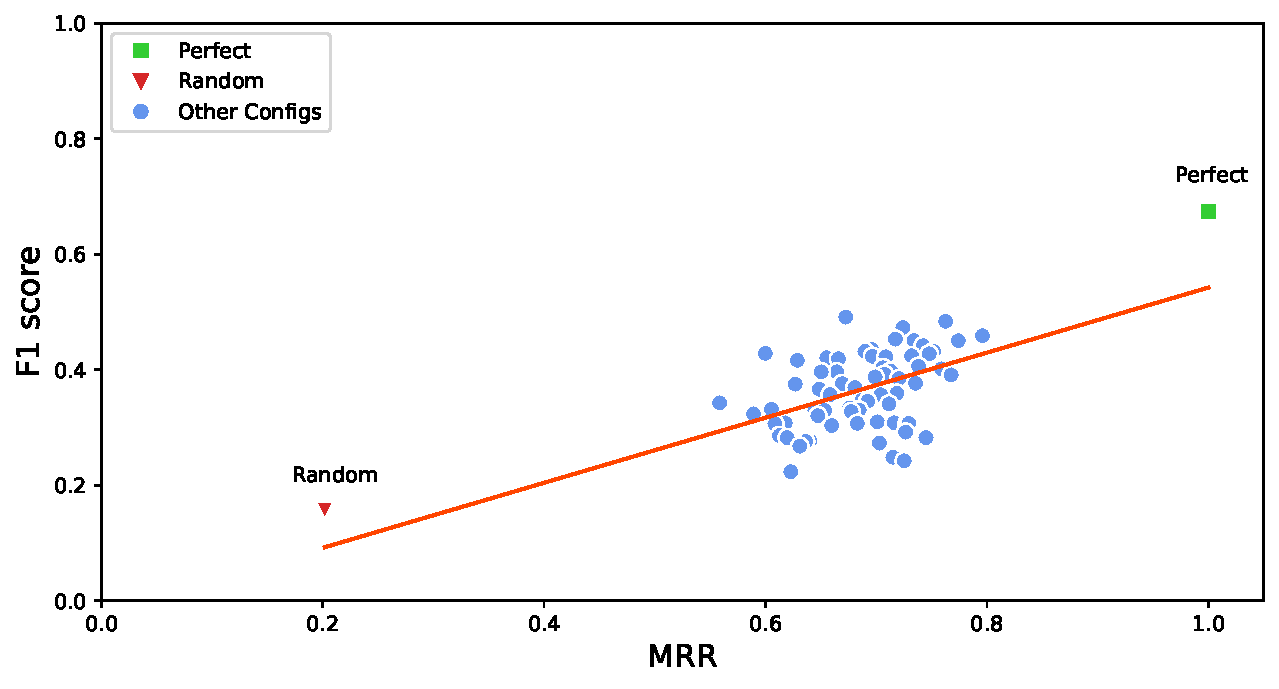
\includegraphics[width=1\linewidth]{images/MRR_craftdroid_all_oracle_included.pdf}
		\caption{\craftdroid as selector}
		\label{fig:MRR_craftdroid_all_oracle_full}
	\end{subfigure}%
	\begin{subfigure}{.5\textwidth}
		\centering
		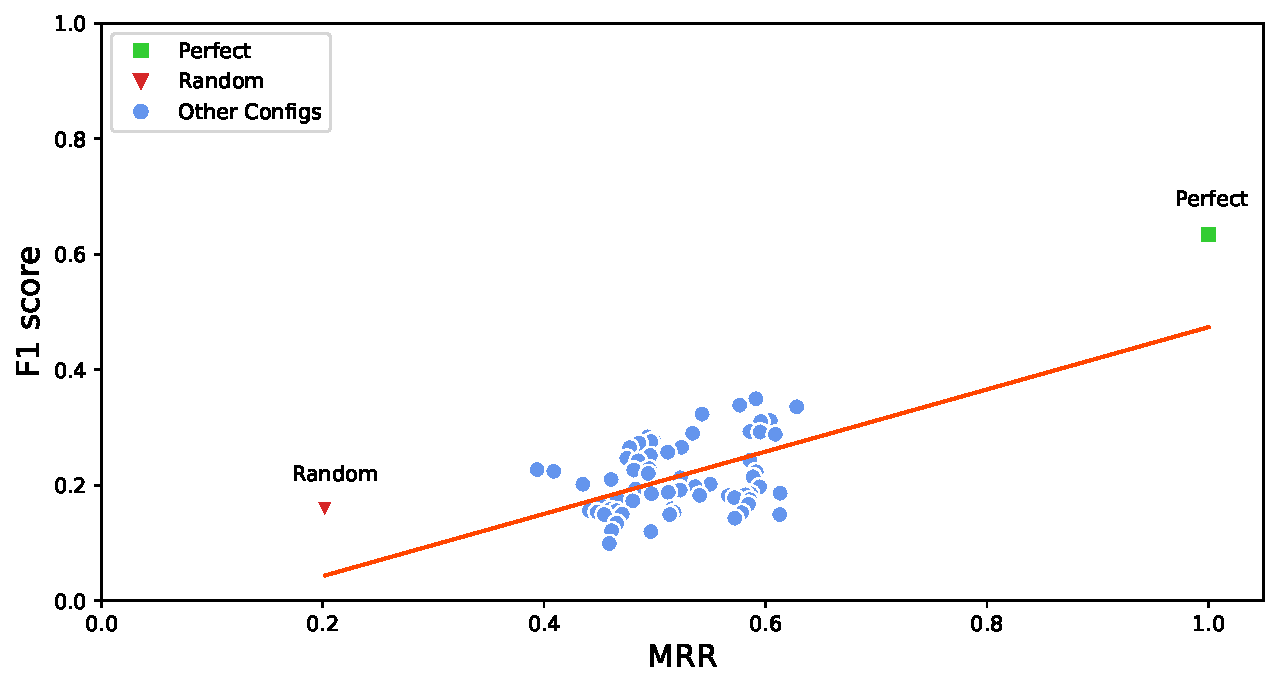
\includegraphics[width=1\linewidth]{images/MRR_atm_atm_oracle_included_passfree.pdf}
		\caption{ ATM as selector}
		\label{fig:MRR_atm_atm_oracle_passfree_full.pdf}
	\end{subfigure}
	\caption{Correlation between semantic matching (\mrr) and \testreuse (\fscore) with oracles}
	\label{fig:MRR-F1-scatter}
\end{figure}
